\documentclass[abstracton,12pt]{scrartcl}
    
\usepackage[utf8]{inputenc}
% \usepackage[T1]{fontenc}
\usepackage{fancyhdr}
\usepackage{graphicx}
\usepackage{tikz}
\usepackage{listings}
\usepackage{amssymb}
\usepackage{amsfonts}
\usepackage{amsmath}
\usepackage{amsthm}
\usepackage{pdfpages}
\usepackage{forest}
\usepackage{multicol}
\usepackage{varwidth}
\usepackage{verbatim}
\usepackage{cleveref}
\usepackage{minted}
\usepackage[ruled,vlined]{algorithm2e}
\usepackage{caption}
\usepackage{subcaption}
\usepackage{soul}
\usepackage{microtype}
\usepackage{pgfplots}
% \usepackage{ulem}
% \usepackage{ifthen}
% \usepackage{wrapfig}
% \usepackage{geometry}
% \usepackage{titlesec}

\forestset{qtree/.style={for tree={parent anchor=south, child anchor=north,align=left,inner sep=0pt}}}
\graphicspath{ {images/} }
\pgfplotsset{yticklabel style={text width=2.5em,align=right}}
% \setlength{\multicolsep}{6.0pt plus 2.0pt minus 1.5pt}% 50% of original values
% \titleformat{\chapter}{}{\thechapter}{}{}
% \titlespacing{\chapter}{-100pt}{-100pt}{-100pt}

% --------- 

\titlehead{Department of Informatics, University of Zürich}
\subject{\vspace*{2cm}MSc Basismodul}
\title{The Adaptive Radix Tree}
\author{
    Rafael Kallis\\[-5pt]
    \scriptsize Matrikelnummer: 14-708-887\\[-5pt]
    \scriptsize Email: \texttt{rk@rafaelkallis.com}
}
\date{\vspace*{2cm}September 18, 2018}
\publishers{
    \small supervised by Prof.\ Dr.\ Michael\ Böhlen and Kevin\ Wellenzohn \\[5cm]
    \begin{tikzpicture}[overlay]
    \node at (-3,-3) {
\includegraphics[height=1.5cm]{IFIlogo}};
    \node at (7,-3) {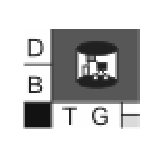
\includegraphics[height=1.5cm]{dbtgBW}};
    \end{tikzpicture}
}

% \dedication{dedicated to xxx}

% --------- 

\theoremstyle{definition}

\newtheorem{definition}{Definition}
% \newtheorem{figure}{Figure}
\newtheorem{example}{Example}
% \newtheorem{theorem}{Theorem}
% \newtheorem{lemma}{Lemma}

\crefname{algocfline}{algorithm}{algorithms}
\Crefname{algocfline}{Algorithm}{Algorithms}

\crefname{figure}{Fig.}{Figs.}
\Crefname{figure}{Figure}{Figures}

\crefname{example}{Ex.}{Ex.}
\Crefname{example}{Example}{Examples}

% \newenvironment{proof}
%     {\noindent{\bf Proof:\rm}}{\hfill$\Box$\vspace{\medskipamount}}

\newenvironment{centerverbatim}{\par\centering\varwidth{\linewidth}\verbatim}
    {\endverbatim\endvarwidth\par}

\def\bbbr{{\rm I\!R}}
\def\bbbm{{\rm I\!M}}
\def\bbbn{{\rm I\!N}}
\def\bbbz{{\rm I\!Z}}

% --------- 

\begin{document}

\maketitle

% \chapter*{Acknowledgements}

% \begin{abstract}
%   ...
% \end{abstract}

% \chapter*{Zusammenfassung}

% \tableofcontents
% \listoffigures
% \listoftables

\newpage
\section{Introduction}

% Main-Memory Databases increasingly become a viable option for many applications
% due to the considerably faster access times and increasing capacities of 
% volatile memory in comparison to secondary storage.

The goal of this project is to study and implement the Adaptive Radix Tree 
(ART), as proposed by Leis et al.\ \cite{leis2013adaptive}.
% ART is an in-memory data structure which efficiently stores and retrieves data.
ART, which is a trie based data structure, achieves its performance, and space
efficiency, by compressing the tree both vertically, i.e., if a node has no 
siblings it is merged with its parent, and horizontally, i.e., uses an array
which grows as the number of children increases.
Vertical compression reduces the tree height and horizontal compression
decreases a node's size.

% The goal of this project is to study and implement ART, as proposed by 
% \cite{leis2013adaptive}. 
In \Cref{sec:art} we describe how ART is constructed by applying 
vertical and horizontal compression to a trie.
Next, we describe the point query procedure, as well as 
key deletion in \Cref{sec:algorithms}.
Finally, a benchmark of ART, a red-black tree and a hashtable
is presented in \Cref{sec:benchmarks}.

\section{Background - Tries}\label{sec:preliminaries}

A trie \cite{fredkin1960trie} is a hierarchical data structure which
stores key-value pairs. Tries can answer both point and range queries 
efficiently since keys are stored in lexicographic order.
Unlike a comparison-based search tree, a trie does not store keys in nodes.
Rather, the digital representation of a search key is split into partial
keys used to index the nodes. When 
constructing a trie from a set of keys, all insertion orders result in the 
same tree. Tries have no notion of balance and therefore do not require 
rebalancing operations.

Keys are split into partial keys of $s$ bits each, where $s$ is called 
\textit{span}. Inner nodes have  $2^s$ child pointers 
(possibly \texttt{null}), one for each possible $s$-bit sequence. During tree
traversal, we descend down to the child node identified by the $d$-th
$s$-bit partial key of the search key, where $d$ is the depth of the current 
node.  Using an array of $2^s$  pointers, this lookup can be done without any 
additional comparison. 

\Cref{fig:span1,fig:span2} depict tries storing the 
8-bit keys ``$01000011$'', ``$01000110$'' and ``$01100100$'' with 
$s \in \{1,2\}$. Nodes with \texttt{\$} are terminator nodes and are used
to indicate the end of a key. Span $s$ is critical for the performance of the 
trie because $s$ determines the height of the trie. When a trie's height
increases, performance deteriorates as more nodes have to be traversed during
a search. We observe that by increasing the span, we decrease the tree height. 
A trie storing $k$ bit keys has $\lceil \frac{k}{s} \rceil$ levels of nodes.
As a consequence, point queries, insertions and deletions have 
$O(k)$ complexity because a trie cannot have a height greater than the length
of keys it stores.

Span $s$ also determines the space consumption of the tree.
A node with span $s$ requires $2^s$ pointers. 
An apparent trade off exists between tree height versus space efficiency that
depends on $s$. Increasing $s$ yields a decrease in the tree's height, 
resulting in faster lookups because less nodes are traversed. On the other
hand, by increasing $s$, nodes require to store more child pointers. Every
increment in $s$ halves the height of the tree but doubles the amount of 
child pointers of each node. Generally, increasing $s$ yields an increase to
the space consumption of a trie.

\begin{figure}[h]
  \centering
  \begin{subfigure}[b]{0.4\textwidth}
    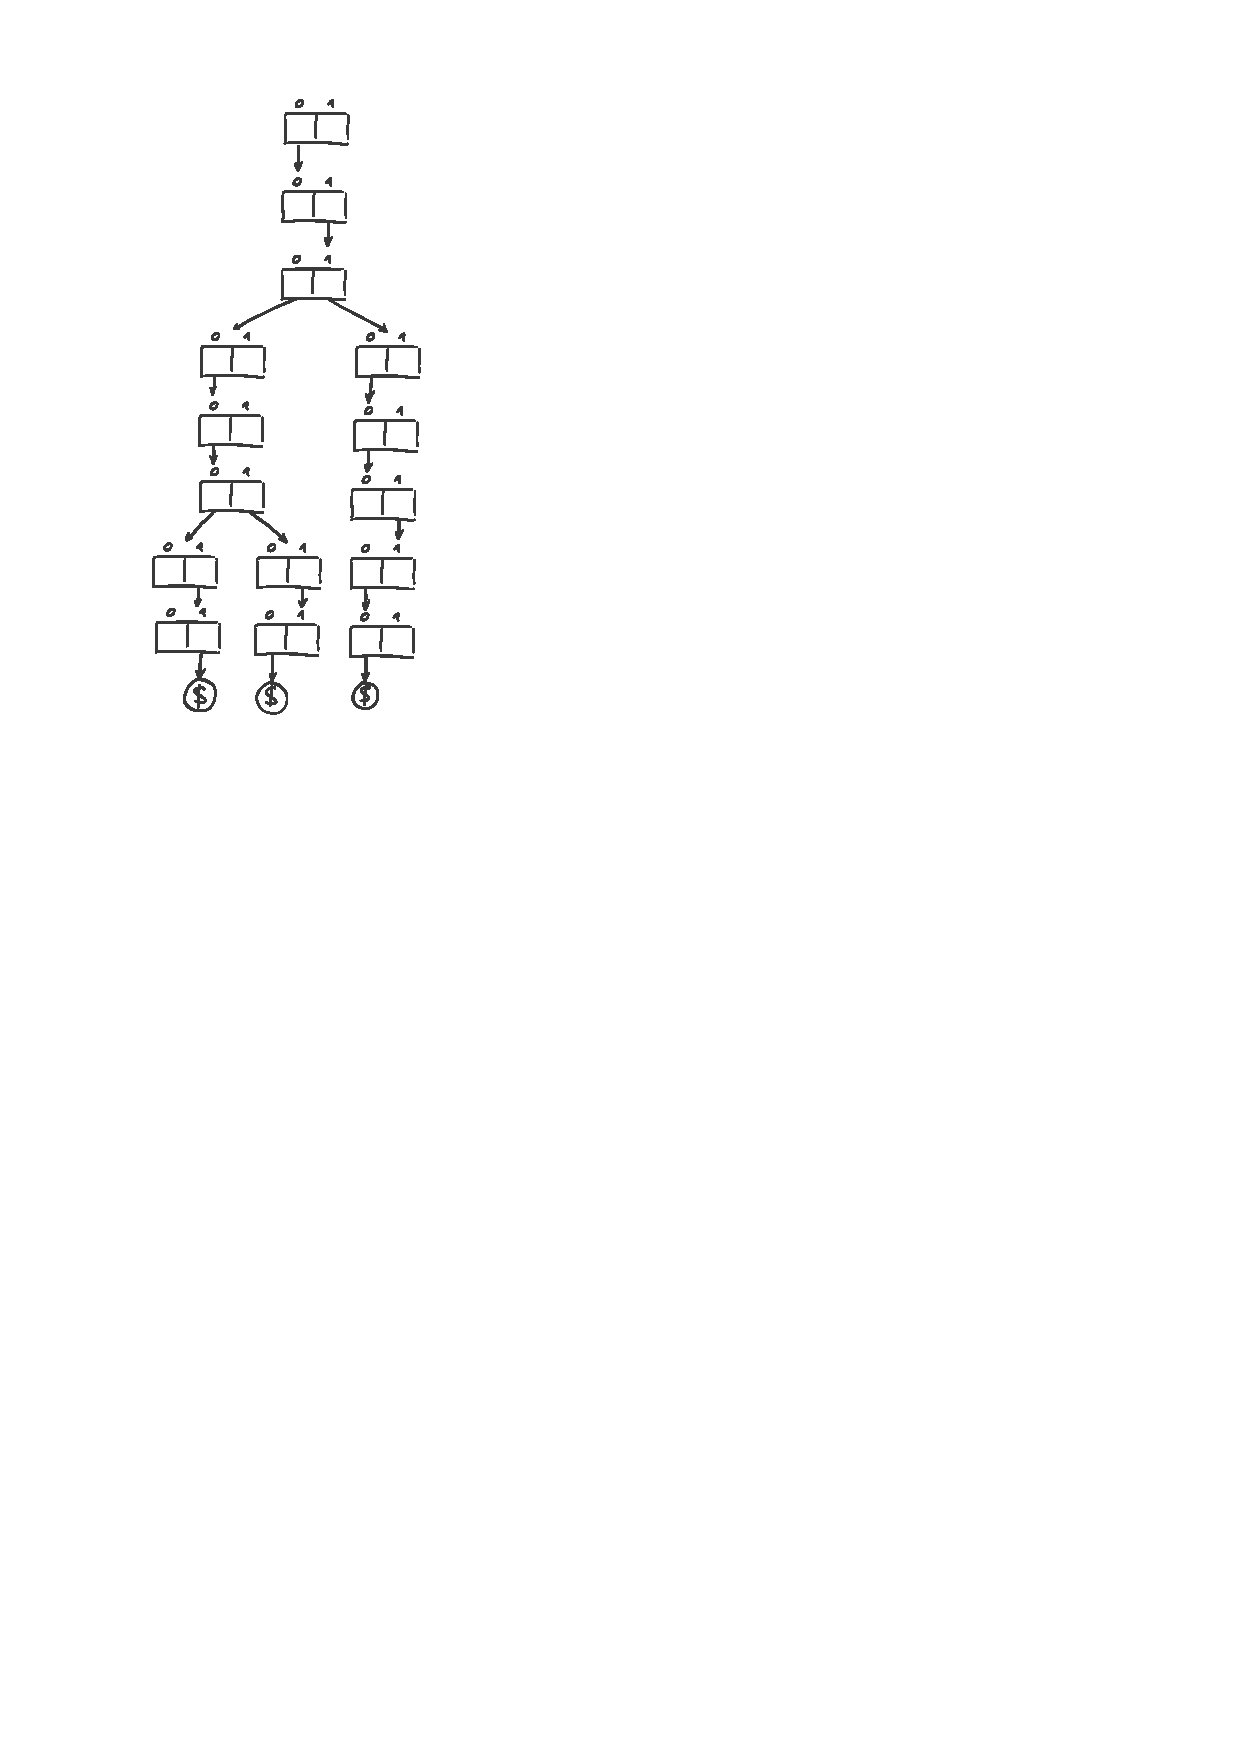
\includegraphics[height=10cm,trim={2cm 17.5cm 2.5cm 1.5cm},clip]{trie_s1_draw}
    \caption{$s=1$}
    \label{fig:span1}
  \end{subfigure}
  \begin{subfigure}[b]{0.55\textwidth}
    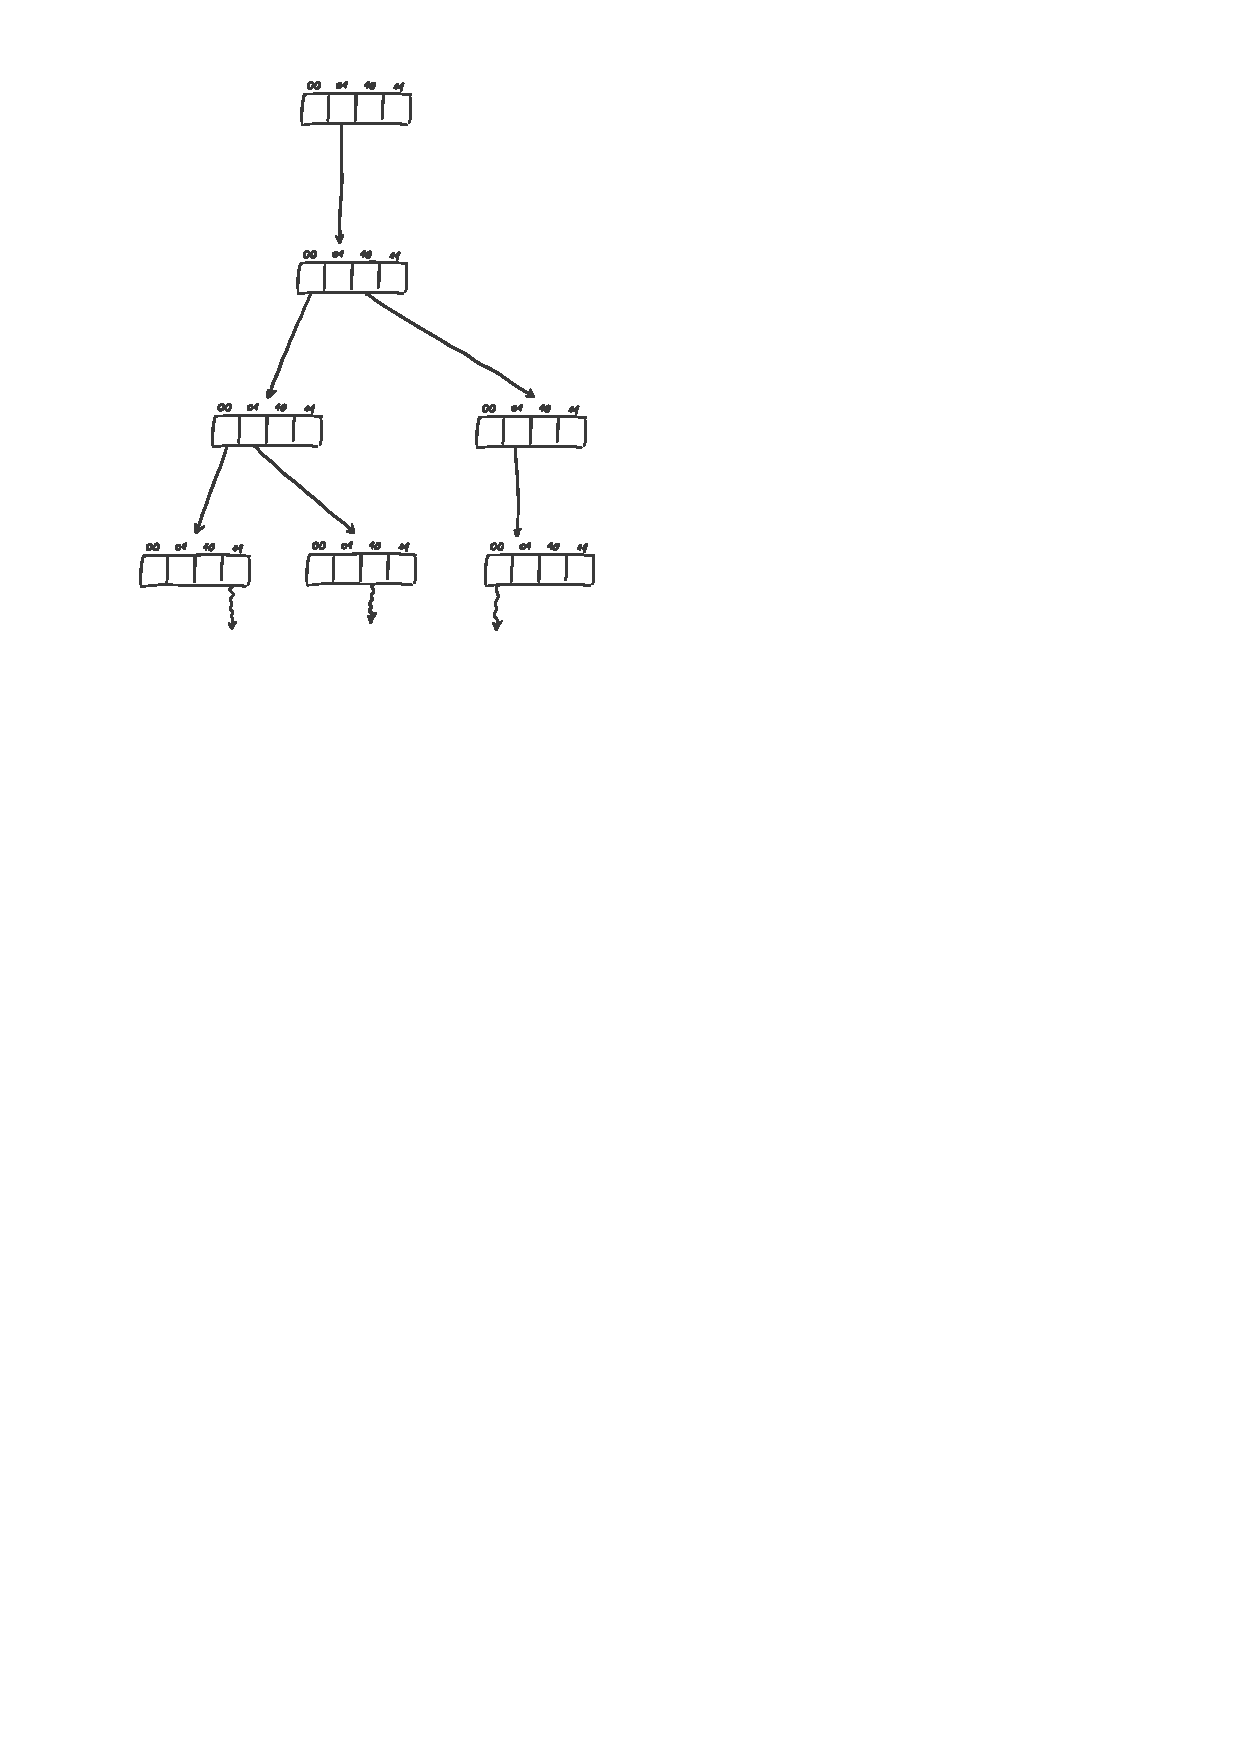
\includegraphics[height=10cm,trim={2cm 18.5cm 2.5cm 0.5cm},clip]{trie_s2_draw}
    \caption{$s=2$}
    \label{fig:span2}
  \end{subfigure}
  \caption{
    Tries with span $s \in \{1,2\}$ storing keys ``$01000011$'', ``$01000110$''
    and ``$01100100$''.
  }
\end{figure}

\newpage

\section{Adaptive Radix Tree (ART)}\label{sec:art}

The \textit{Adaptive Radix Tree} (ART) is a space efficient trie, which
achieves its low memory consumption using \textit{vertical} and 
\textit{horizontal} compression. Using vertical compression, ART reduces
the tree height significantly by merging parent nodes with child nodes
under certain circumstances. Horizontal compression reduces the amount
of space required by each node depending on the number of child nodes.

\subsection{Vertical (Prefix) Compression}\label{sec:vertical-compression}

When storing long keys, chains of nodes start to form where each node only
has a single child. (e.g.\ the trie in \Cref{fig:span1} stores ``01100100'',
we see a chain of five nodes).
As a consequence, space is wasted as many nodes
with little actual content are kept and traversals are slowed down because
many nodes are traversed. Space wasting is further amplified with sparse
datasets or a small span.

Morrison introduced \textit{Patricia}~\cite{morrison1968patricia}. 
Patricia is a space-optimized trie in which
each node with no siblings is merged with its parent, i.e., inner nodes
are only created if they are required to distinguish at least two leaf nodes. 
Doing so, chains caused by long keys are eliminated, which make tries 
space-inefficient. Morrison's Patricia tree is a bitwise trie, i.e.,
has a span $s=1$, but the technique can be applied to tries with any span,
although it becomes less effective as span $s$ increases.
We refer to this technique as \textit{vertical compression}.

Leis et al.\ mention three approaches to deal with vertical compression:
\begin{itemize}
  \item Pessimistic: We store an additional variable, called \texttt{prefix},
    inside each node. This variable stores the concatenation of partial keys
    of descendants that were eliminated because they had no siblings. During
    lookup, \texttt{prefix} is compared to the search key before proceding to
    the next child. If a mismatch occurs, then the key is not contained and
    the search terminates returning \texttt{null}.
    \Cref{fig:vertical-compression} depicts two tries, one 
    with and one without vertical compression using the pessimistic approach.
    We observe that nodes with no siblings, color coded red, are eliminated 
    and their partial key is appended to the parent's prefix (highlighted in
    gray).

  \item Optimistic: Only the number of compressed nodes is stored. Lookups
    skip this number of partial keys without comparing them to the search
    key. Full keys are required to be stored on leaf nodes. When a lookup 
    arrives to a leaf node, its key must be compared to the search key.
    In case of a mismatch, the search key is not contained and the search is 
    terminated returning \texttt{null}.

  \item Hybrid: We store the number of compressed nodes and a static, 
    fixed-size array in order to store a part of the compressed path. If the 
    number of compressed nodes exceeds the size of the array, the optimistic 
    strategy is used instead.
\end{itemize}

\begin{figure}[h]
  \begin{footnotesize}
    \begin{multicols}{2}
      \noindent
      \begin{flushright}
      \framebox(160,160){
        \begin{forest}
          [,circle,draw
            [,circle,draw,red, edge label={node[midway,right,font=\footnotesize]{$01$}}
              [,circle,draw, edge label={node[midway,left,font=\footnotesize]{$00$}}
                [,circle,draw, edge label={node[midway,left,font=\footnotesize]{$00$}}
                  [\texttt{\$},circle,draw,red,inner sep=0,edge label={node[midway,left,font=\footnotesize]{$11$}}]
                ]
                [,phantom]
                [,circle,draw, edge label={node[midway,right,font=\footnotesize]{$01$}}
                  [\texttt{\$},circle,draw,red,inner sep=0,edge label={node[midway,right,font=\footnotesize]{$10$}}]
                ]
              ]
              [,phantom]
              [,phantom]
              [,circle,draw, edge label={node[midway,right,font=\footnotesize]{$10$}}
                [,circle,draw,red, edge label={node[midway,right,font=\footnotesize]{$01$}}
                  [\texttt{\$},circle,draw,red,inner sep=0,edge label={node[midway,right,font=\footnotesize]{$00$}}]
                ]
              ]
            ]
          ]
        \end{forest}
      }
      \hspace{5mm}
      \end{flushright}
      ~

      \begin{flushleft}
      \hspace{5mm}
      \framebox(160,160){
        \begin{forest}
          [,circle,draw
            [,circle,draw, edge label={node[midway,left,font=\footnotesize]{$00$}}
              [\texttt{\$},circle,draw,inner sep=0,edge label={node[midway,left,font=\footnotesize]{$00$}}]{
                \draw[gray] (.east)--++(0.5em,0em)
                  node[anchor=west,gray]{11};
              }
              [,phantom]
              [\texttt{\$},circle,draw,inner sep=0,edge label={node[midway,right,font=\footnotesize]{$01$}}]{
                \draw[gray] (.east)--++(0.5em,0em)
                  node[anchor=west,gray]{10};
              }
            ]
            [,phantom]
            [,phantom]
            [\texttt{\$},circle,draw,inner sep=0,edge label={node[midway,right,font=\footnotesize]{$10$}}]{
              \draw[gray] (.east)--++(0.5em,0em)
                node[anchor=west,gray]{0100};
            }
          ]{
            \draw[gray] (.east)--++(0.5em,0em)
              node[anchor=west,gray]{01};
          }
        \end{forest}
      }
      \end{flushleft}
    \end{multicols}
  \end{footnotesize}
  \caption{
    Tries with span $s=2$ storing keys ``$01000011$'', ``$01000110$''
    and ``$01100100$''. The trie on the right incorporates (pessimistic)
    vertical compression. Red nodes indicate nodes which get eliminated under
    vertical compression. Gray strings represent the value of the prefix 
    variable.
  }
  \label{fig:vertical-compression}
\end{figure}

\newpage

\subsection{Horizontal Compression (Adaptive Nodes)}\label{sec:horizontal-compression}

With large values of span $s$, an excessive amount of space is sacrificed
to achieve a smaller tree height. Larger nodes means space is allocated for 
pointers which keep references to child nodes, even if they are unused.

In order to reduce space needed to keep
such references, Leis et al.\ propose \textit{Adaptive Nodes} 
\cite{leis2013adaptive}, which make use of dynamic data structures 
instead of static arrays for child node bookkeeping. Doing so, we allocate 
less space when the number of children is small and add more 
space if required, i.e., more children are added.
We refer to this technique as \textit{horizontal compression}.
Leis et al.\ fix the span $s=8$, i.e., partial keys are 1 byte
long and therefore each node can have up to $2^8 = 256$ children.

When applying horizontal compression, a node is in one of four configurations, 
depending on the number of child nodes. Each of the four configurations is 
optimized for a different amount of children.
When keys are inserted/deleted, the nodes are adapted accordingly.
The most compact configuration 
is called \texttt{Node4} which can carry up to four children. 
In the same manner, we also have \texttt{Node16}, \texttt{Node48} 
and \texttt{Node256}. All nodes have a header which stores the node type,
the number of children and the prefix variable, which contains the compressed
path (c.f.\ \Cref{sec:vertical-compression}).

\begin{table}[h]
  \centering
  \begin{tabular}{ l|r|r } 
    Type & Children & Space (bytes) \\
    \hline
    \texttt{Node4} & 2-4 & $h + 4 + 4 \cdot 8 = h + 36$ \\ 
    \texttt{Node16} & 5-16 & $h + 16 + 16 \cdot 8 = h + 144$ \\ 
    \texttt{Node48} & 17-48 & $h + 256 + 48 \cdot 8 = h + 640$ \\ 
    \texttt{Node256} & 49-256 & $h + 256 \cdot 8 = h + 2048$ 
  \end{tabular}
  \caption{Space consumption for each inner node type. $h$ is equal to
    the size of the header.}
  \label{tbl:node-sizes}
\end{table}

We now describe the structure of each of the four configurations.
\Cref{tbl:node-sizes} shows the space consumption for each inner node type.
Note that $h$ is equal to the header's size.
\Cref{fig:horizontal-compression} illustrates the state of a node
for each node type, when storing the partial keys $65$ (``01000001''), 
$82$ (``01010010''), $84$ (``01010100'') and pointers to their corresponding 
child nodes $\alpha$, $\beta$, $\gamma$. Note that $\varnothing$ represents 
a \texttt{null} pointer.

A node of type \texttt{Node4} contains two 4-element arrays, one called
``partial keys'' and one called ``children''.
The ``partial keys'' array holds partial keys of the child nodes. 
The ``children'' array, holds pointers to the child nodes.
Partial keys and pointers are stored at corresponding positions in their
respective arrays and the partial keys are sorted.

A node of type \texttt{Node16} is structured similarly
to \texttt{Node4}, the only difference being the lengths of the two static 
arrays, which are 16 each.

An instance of \texttt{Node48} contains a 256-element array named 
``indexes'' ($256$ bytes) and a 48-element array called ``children''
($48 \cdot 8$ bytes).
Partial keys are stored implicitly in ``indexes'', i.e., 
can be indexed with partial key bytes directly.
As the name suggests, ``indexes'' stores the index of a child
node inside the ``children'' array. $48$ is a special value in the
``indexes'' array and is used to signal that the partial key
does not exist.

Finally, a node of type \texttt{Node256} contains an array of
256 pointers which can be indexed with partial key bytes directly.
Child nodes can be found with a single lookup.

\begin{figure}[H]
  \centering
  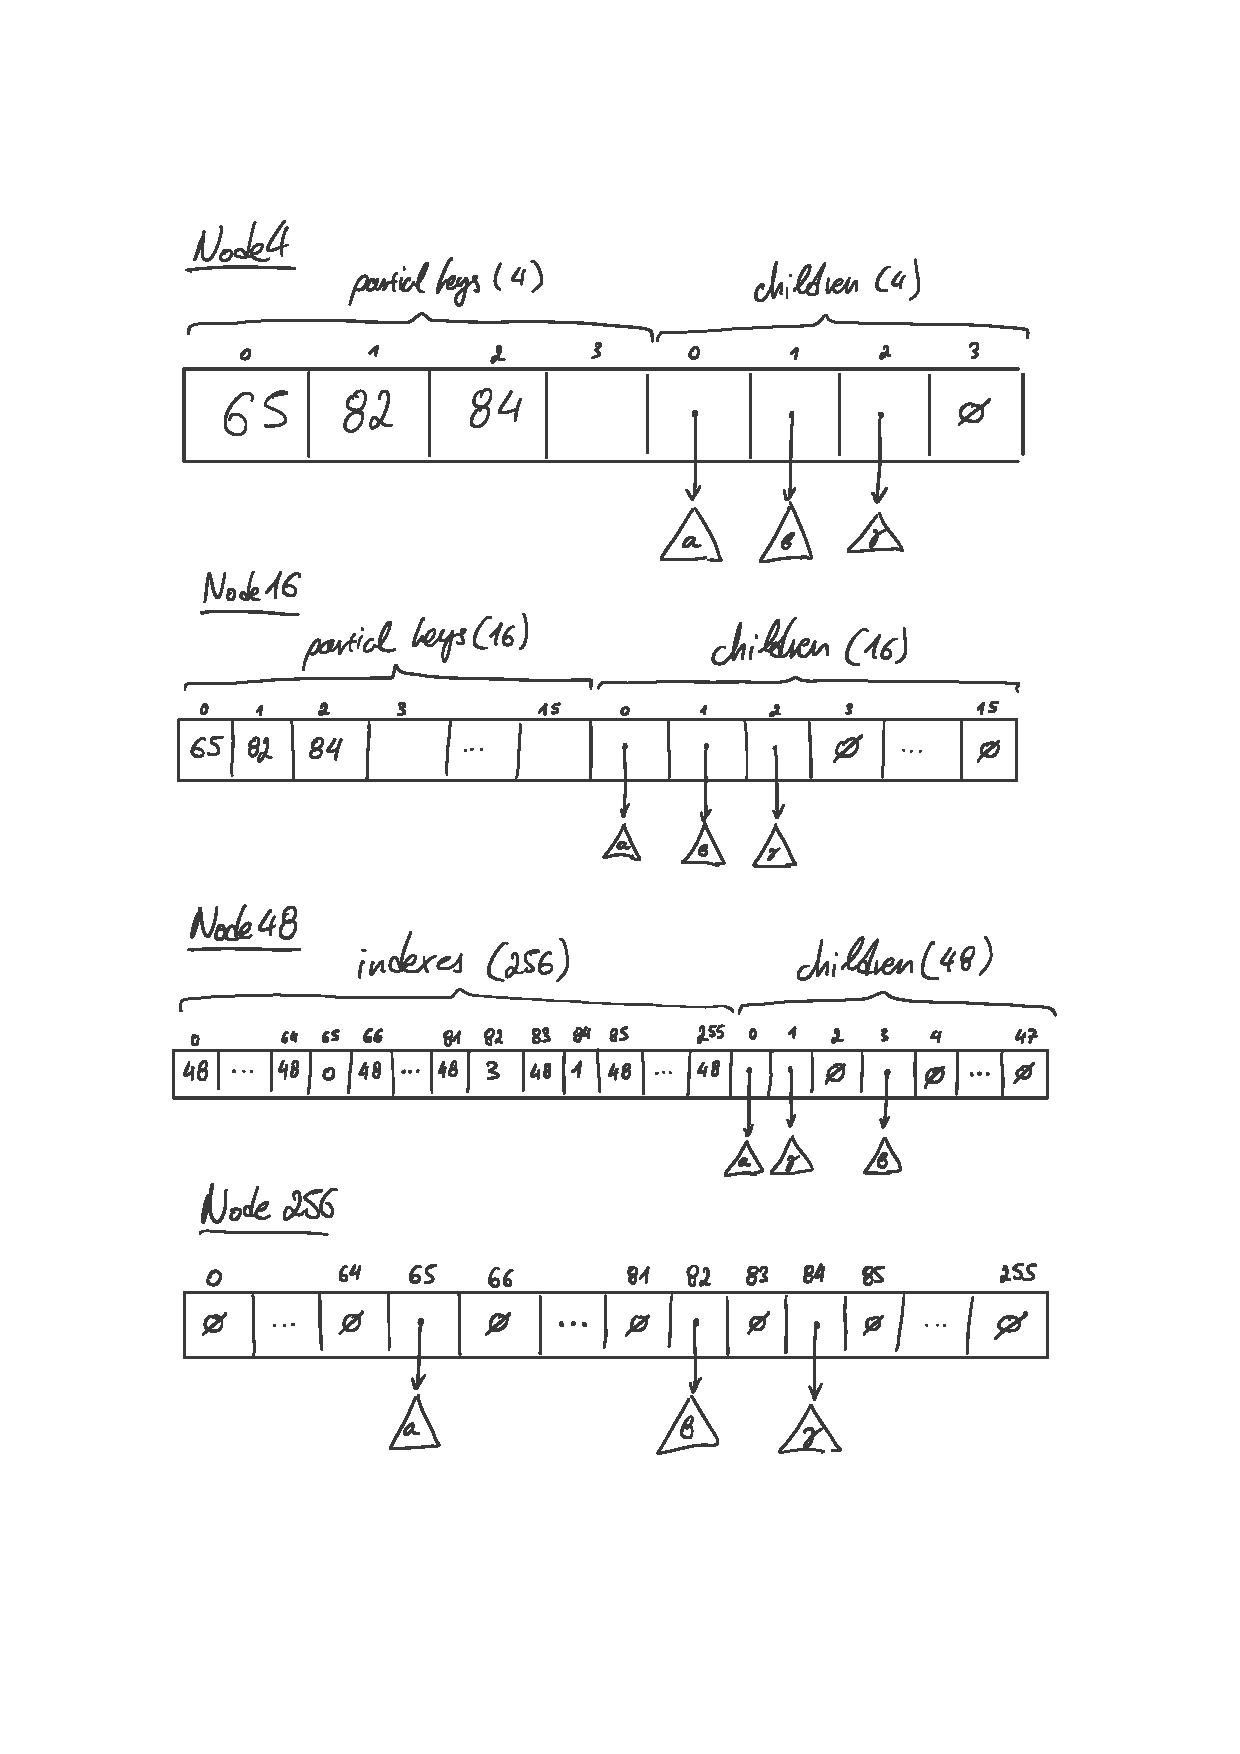
\includegraphics[height=20cm,trim={2.5cm 5cm 2.5cm 3.5cm},clip]{art_nodes_draw}
  \caption{
    When horizontal compression is applied, a node is in one of four 
    configurations, namely \texttt{Node4}, \texttt{Node16}, \texttt{Node48} 
    and \texttt{Node256}.
    Each of the four configurations is optimized for a different number of 
    child nodes. We store the partial keys $65$, $82$, $84$ and their 
    corresponding child nodes $\alpha$, $\beta$, $\gamma$ in an instance
    of each node type. Note that $\varnothing$ represents a \texttt{null} 
    pointer.
  }
 \label{fig:horizontal-compression}
\end{figure}

\newpage

\section{Algorithms}\label{sec:algorithms}

\vspace{-2mm}
We will now describe how two fundamental operations, namely
point query and deletion are implemented in ART.
Range queries and insertions are similar and are omitted for brevity.

Note that our implementation uses
\textit{single-value leaves} (c.f.\ Leis et al.), 
i.e., values are stored using an additional leaf node type, conveniently
called \texttt{Node0}, which stores one value. \texttt{Node0} is equivalent to
a terminator node mentioned in \Cref{sec:preliminaries}. Additionally, we utilize
pessimistic vertical compression (c.f.\ \Cref{sec:vertical-compression}),
i.e., each inner node stores the entire compressed path inside the 
\texttt{prefix} variable using a variable length partial key array. 
We present our implementations below.

\vspace{-4mm}
\subsection{Point Query}\label{sec:point-query}

\vspace{-1mm}
The code fragment in \Cref{algo:point-query} shows the implementation of a 
point query on ART in C++. Method \texttt{get} accepts a key and its length
as an argument and returns a pointer to the value associated with the given 
key, or \texttt{null} if the key is not found.

In lines 2-3 we declare and initialize a pointer, \texttt{cur}, which references
the current node during tree traversal, \texttt{child} which references 
\texttt{cur}'s child and \texttt{depth}, which holds the depth
of the current node. We now enter a loop in which we check if \texttt{cur} 
references \texttt{null} during the beginning of each iteration, and if so, 
the search key is not contained and we return \texttt{null}.

In lines 5-8 we check if a prefix mismatch occurs. This step is required
because of vertical compression (c.f.\ \Cref{sec:vertical-compression}).
If a prefix mismatch is discovered, \texttt{null} is returned. Method 
\texttt{check\_prefix} is a member of the \texttt{node} class which
determines the number of matching bytes between \texttt{cur}'s prefix
and \texttt{key} w.r.t.\ the current depth, e.g., given a node with prefix
``\texttt{abbd}'', a search key ``\texttt{aaabbbccc}'' and depth $2$, then
\texttt{check\_prefix} returns $3$, since the $4$-th byte of the prefix
(`\texttt{d}'), does not match the (depth + $4$)-th byte of the search key
(`\texttt{b}').

Lines 9-12 check for an exact match of the key at the current node. If so,
we return the value of the current node. Finally, we traverse to the next child
node. Variable \texttt{depth} is adjusted according to the number of nodes 
merged due to vertical compression. We lookup the next child node, which is 
assigned to \texttt{cur}. If no such child exists, the search key does not 
exist and \texttt{null} is returned.

\vspace{-2mm}

\begin{figure}[H]
  \begin{minted}[numbers=left,frame=single,fontsize=\scriptsize]{c++}
template <class T> T * art<T>::get(const char *key, const int key_len) const {
  node<T> *cur = root_, **child = nullptr;
  int depth = 0;
  while (cur != nullptr) {
    if (cur->prefix_len_ != cur->check_prefix(key + depth, key_len - depth))
      /* prefix mismatch */
      return nullptr;
    if (cur->prefix_len_ == key_len - depth)
      /* exact match */
      return cur->value_;
    child = cur->find_child(key[depth + cur->prefix_len_]);
    cur = child != nullptr ? *child : nullptr;
    depth += cur->prefix_len_ + 1;
  }
  return nullptr;
}
  \end{minted}
  \vspace{-6mm}
  \caption{Point query implemented in C++.}
  \label{algo:point-query}
  \vspace{-7mm}
\end{figure}

\newpage

\subsection{Deletion}\label{sec:deletion}

\Cref{algo:deletion} presents our implementation of key deletion on ART in C++.
During deletion, the leaf node identified by the search key is removed from an
inner node, which is shrunk if necessary. 
If the leaf to remove only has one sibling, vertical
compression is applied. We assume all leaf nodes are of type \texttt{Node0}.

In lines 3-5, we declare and initialize two pointers, \texttt{cur} and
\texttt{par} which reference the current and parent node during tree traversal.
Variable \texttt{cur\_partial\_key} holds the partial key which indexes the
current node in the parent's child lookup table.
Variable \texttt{depth} holds the depth of the current node.
We loop until \texttt{cur} references either the right leaf node or
\texttt{null}. In the latter case, the is not contained and \texttt{null} is 
returned.

Line 12 checks if \texttt{cur} is a leaf node, i.e.\ the node that contains 
the search key has been found. If that is not the case, we
continue descending down (lines 57-60). Given \texttt{cur} is a leaf, one
of three cases is possible depending on \texttt{cur}'s siblings:

\begin{itemize}
  \item If \texttt{cur} has \textit{no siblings} (lines 18-24), \texttt{cur}
    must be the root. We delete \texttt{cur} and set the root to \texttt{null}.

  \item If \texttt{cur} has \textit{one sibling} (lines 24-48), vertical
    compression is applied, effectively removing both \texttt{cur} and its
    parent \texttt{par}. During this process, \texttt{par}'s prefix,
    as well as the sibling's partial key, are prepended to the sibling's
    prefix.

    Lines 26-30 search for \texttt{cur}'s sibling. Next, lines 34-39 assign 
    the concatenation of: 1) \texttt{par}'s prefix, 2) the sibling's 
    partial key and 3) the sibling's old prefix, to the sibling's new prefix.

    Lines 40-45 perform cleanup operations, freeing memory previously allocated
    by the sibling's old prefix, \texttt{cur}, \texttt{cur}'s prefix,
    \texttt{par} and \texttt{par}'s prefix. 
    
    Finally, \texttt{sibling} replaces the parent (line 46).

  \item If \texttt{cur} has \textit{more than one sibling} (lines 48-54),
    we remove \texttt{cur} from its parent \texttt{par} and shrink
    \texttt{par} if needed (c.f.\ \Cref{sec:horizontal-compression}).
\end{itemize}

Finally, the value associated with the search key is returned (in case the
method callee has to free resources).

\begin{figure}[H]
  \begin{minted}[numbers=left,frame=single,fontsize=\scriptsize]{c++}
template <class T> T *art<T>::del(const char *key, const int key_len) {
  if (root_ == nullptr) { return nullptr; }
  node<T> **par = nullptr, **cur = &root_;
  char cur_partial_key;
  int depth = 0;

  while (cur != nullptr) {
    if ((**cur).prefix_len_ != (**cur).check_prefix(key + depth, key_len - depth)) {
      /* prefix mismatch */
      return nullptr;
    }
    if (key_len == depth + (**cur).prefix_len_) {
      /* exact match */
      T *value = (**cur).value_;
      (**cur).value_ = nullptr;
      int n_siblings = par != nullptr ? (**par).n_children() - 1 : 0;

      if (n_siblings == 0) {
        /* cur is root */
        if ((**cur).prefix_ != nullptr) { delete[](**cur).prefix_; }
        delete (*cur);
        *cur = nullptr;

      } else if (n_siblings == 1) {
        /* find sibling and apply vertical compression */
        char sibling_partial_key = (**par).next_partial_key(0);
        if (sibling_partial_key == cur_partial_key) {
          sibling_partial_key = (**par).next_partial_key(cur_partial_key + 1);
        }
        node<T> *sibling = *(**par).find_child(sibling_partial_key);
        char *old_prefix = sibling->prefix_;
        int old_prefix_len = sibling->prefix_len_;
        /* compute new prefix of sibling */
        sibling->prefix_ = new char[(**par).prefix_len_ + 1 + old_prefix_len];
        sibling->prefix_len_ = (**par).prefix_len_ + 1 + old_prefix_len;
        std::memcpy(sibling->prefix_, (**par).prefix_, (**par).prefix_len_);
        sibling->prefix_[(**par).prefix_len_] = sibling_partial_key;
        std::memcpy(sibling->prefix_ + (**par).prefix_len_ + 1, old_prefix,
               old_prefix_len);
        if (old_prefix != nullptr) { delete[] old_prefix; }
        /* remove cur and par */
        if ((**cur).prefix_ != nullptr) { delete[](**cur).prefix_; }
        delete (*cur);
        if ((**par).prefix_ != nullptr) { delete[](**par).prefix_; }
        delete (*par);
        *par = sibling;

      } else if (n_siblings > 1) {
        /* remove cur */
        if ((**cur).prefix_ != nullptr) { delete[](**cur).prefix_; }
        delete (*cur);
        (**par).del_child(cur_partial_key);
        if ((**par).is_underfull()) { *par = (**par).shrink(); }
      }
      return value;
    }
    cur_partial_key = key[depth + (**cur).prefix_len_];
    depth += (**cur).prefix_len_ + 1;
    par = cur;
    cur = (**cur).find_child(cur_partial_key);
  }
  return nullptr;
}
  \end{minted}
  \caption{Key deletion implemented in C++.}
 \label{algo:deletion}
\end{figure}

\newpage

\section{Benchmarks}\label{sec:benchmarks}

In this section we compare the performance of ART against the two textbook
data structures red-black tree (RBT) and chained hash table (HT).
We chose RBT to compete against ART because, like ART, RBT is a hierarchical
data structure with sorted keys, and supports answering both point and range
queries efficiently. HT does answer point queries faster but lacks support for
efficient range queries. We use C++ standard library containers 
\texttt{std::map} and \texttt{std::unordered\_map}\footnote{https://en.cppreference.com/w/cpp/container}
which are implementations of RBT and HT, respectively.

Let $k$ be the length of the keys and $n$ be the size of the dataset, then
ART, RBT and HT have an average case complexity of $O(k)$, 
$O(\log{}n)$ and $O(1)$,\footnote{amortized
$O(1)$ during insertion and deletion.} respectively, 
for point queries, insertion and deletion. ART's and RBT's big-O complexities are
incomparable, as one depends on the length of the keys and the other on the 
size of the dataset $n$. HT, with an average case 
complexity of $O(1)$, should outperform ART and RBT.

We first conduct a series of microbenchmarks in order to assess point query,
insertion and deletion performance and then conduct an experiment in order
to measure how often vertical compression is applied on ART. 

There are three datasets, i.e., set of keys, used for the benchmarks: a sparse
dataset, a dense dataset and a mixed dataset, called the Dell
dataset~\cite{wellenzohn2017wapi}, with sparse and dense regions. 
A dataset is dense (sparse) if many (few) keys share common prefixes. 

The dataset of size $n = 16$ million is constructed by drawing $n$ uniformly 
distributed 64-bit integers. The dense dataset of size $n$ is constructed 
by picking 64-bit integers from $0$ to $n - 1$ (leading bits are filled with 
zeroes).

\subsection{Microbenchmarks}\label{sec:microbenchmarks}

During the lookup microbenchmark, we execute point queries on an instance
of each of the three data structures (ART, RBT, HT)
containing the same $n=16$ million keys. The keys are sparse (i.e., uniformly
distributed), 64-bit integers. Each key is queried exactly once.
The insertion microbenchmark inserts the same sixteen million sparse 64-bit keys
used previously. Finally, the deletion microbenchmark, structured similar to 
the lookup microbenchmark, attempts to delete every stored key from the data 
structure.

\Cref{fig:lookup-microbenchmark,fig:insertion-microbenchmark,fig:deletion-microbenchmark}
show the results of the three microbenchmarks. ART is positioned in between 
its competitors in all three microbenchmarks and shows a robust performance.
ART's performance depends on key length $k$, but HT does not (constant), which 
explains why ART is slower than HT. Although ART's and RBT's big-O complexities 
are incomparable as the one depends on the key length $k$ and the other on the 
size of the dataset $n$, ART seems to outperform RBT in practice for point 
queries, insertion and deletion.
% We observe that HT is faster than its competitors. As mentioned earlier, HT's
% average case complexity is constant, whereas ART and RBT have an average case
% complexity of $\mathcal{O}(k)$ and $\mathcal{O}(\log{}n)$, respectively.

We also observe that ART performs half as fast compared to HT during the 
lookup microbenchmark, but is as fast as HT during insertion.
We believe this happens because during insertion, HT occasionally 
requires a table resize and full rehash.

\begin{figure}[H]
  \centering
  \begin{subfigure}[b]{0.3\textwidth}
    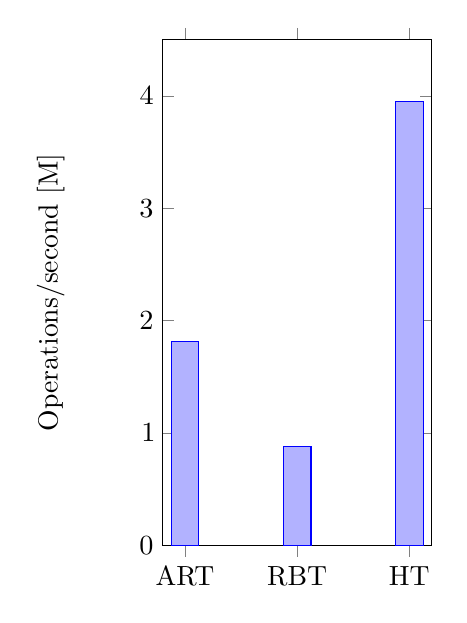
\begin{tikzpicture}
      \begin{axis}[
        ybar,
        symbolic x coords={ART,RBT,HT},
        ylabel=Operations/second {[M]},
        ymax = 4.5,
        ymin = 0,
        width=5cm,
        height=8cm,
        ]
        \addplot coordinates {(ART,1.8100282) (RBT,0.8763096) (HT,3.9497637)};
      \end{axis}
    \end{tikzpicture}
    \caption{Lookup}
    \label{fig:lookup-microbenchmark}
  \end{subfigure}
  \begin{subfigure}[b]{0.3\textwidth}
    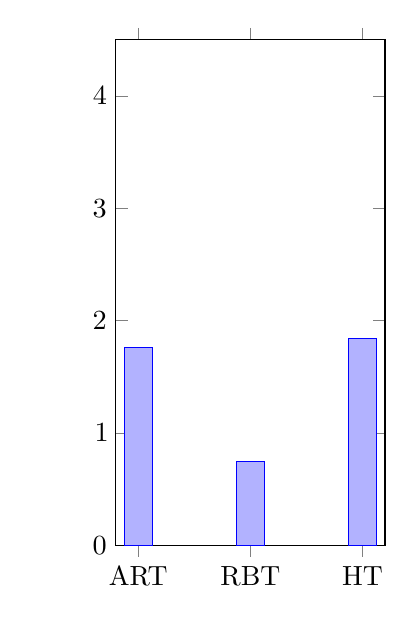
\begin{tikzpicture}
      \begin{axis}[
        ybar,
        symbolic x coords={ART,RBT,HT},
        ymax = 4.5,
        ymin = 0,
        width=5cm,
        height=8cm,
        ]
        \addplot coordinates {(ART,1.7570827) (RBT,0.7479445) (HT,1.8366757)};
      \end{axis}
    \end{tikzpicture}
    \caption{Insertion}
    \label{fig:insertion-microbenchmark}
  \end{subfigure}
  \begin{subfigure}[b]{0.3\textwidth}
    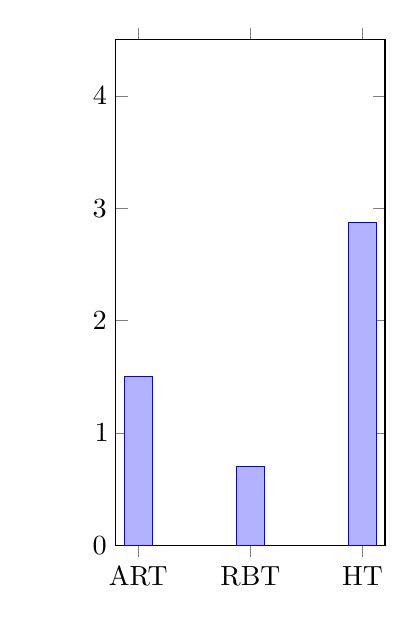
\begin{tikzpicture}
      \begin{axis}[
        ybar,
        symbolic x coords={ART,RBT,HT},
        ymax = 4.5,
        ymin = 0,
        width=5cm,
        height=8cm,
        ]
        \addplot coordinates {(ART,1.4992408) (RBT,0.6993710) (HT,2.8705743)};
      \end{axis}
    \end{tikzpicture}
    \caption{Deletion}
    \label{fig:deletion-microbenchmark}
  \end{subfigure}
  \caption{Lookup, insertion and deletion performance of ART,
  red-black trees (RBT) and hashtables (HT) over the sparse dataset.}
  \label{fig:microbenchmark}
\end{figure}

\vspace{-5mm}

\subsection{Vertical Compression}
\label{sec:compression-benchmark}

Vertical compression is an expensive operation, as it involves structural index
modifications when applied. Such structural index modifications can be
difficult to implement efficiently for concurrency control because 
synchronization of concurrent
transactions is required during such operations~\cite{wellenzohn2017wapi}.
Our last experiment measures how often vertical compression is applied
when we store keys from the sparse, dense and Dell dataset.
As mentioned in \Cref{sec:vertical-compression}, when deleting a node with
a single sibling, the sibling is compressed, i.e., merged with its parent.

Analogously, when inserting a key, if a leaf is encountered or the search key
differs from the compressed path, \textit{expansion} is applied, i.e., a new 
inner node is created above the current node and the compressed paths are 
adjusted accordingly. We report only the number of vertical compressions during
deletion, but found that the number of compressions during deletion equals the 
number of expansions during insertion.

The number of compressions
depends on span $s$. If $s=1$, every node must have exactly one sibling,
and therefore every deletion requires a compression, unless the root is
deleted. ART has a span of $s=8$ and we therefore do not expect a compression 
for every deletion.

Results should vary depending if keys are sparse or dense. Dense keys
yield a higher node fanout which causes fewer compressions.
We therefore expect that having dense keys implies a smaller number
of compressions.

\Cref{fig:compressions-sparse,fig:compressions-paths,fig:compressions-dense} 
depict number of vertical
compressions over number of transactions for the sparse, Dell and dense 
dataset. We observe a linear relation between the two variables. As expected,
dense keys require less compressions compared to sparse keys. That is because
with the dense dataset, ART nodes have a higher fanout. If a node has many children, more
deletions are required until compression is applied.
We also observe that the Dell dataset lies between the sparse and dense
dataset in terms of compressions per operation but tends towards the 
dense dataset.

\begin{figure}[H]
  \centering
  \begin{subfigure}[b]{0.30\textwidth}
    \begin{tikzpicture}
      \begin{axis}[
        xmax=11,
        ymax=4.5,
        xlabel={Operations [M]},
        ylabel=Compressions {[M]},
        height=7cm,
        width=5cm,
        ]
        \addplot table {compressions_sparse.dat};
      \end{axis}
    \end{tikzpicture}
    \caption{Sparse Dataset}
    \label{fig:compressions-sparse}
  \end{subfigure}
  \begin{subfigure}[b]{0.30\textwidth}
    \begin{tikzpicture}
      \begin{axis}[
        xmax=11,
        ymax=4.5,
        xlabel={Operations [M]},
        height=7cm,
        width=5cm,
        ]
        \addplot table {compressions_paths.dat};
      \end{axis}
    \end{tikzpicture}
    \caption{Dell Dataset}
    \label{fig:compressions-paths}
  \end{subfigure}
  \begin{subfigure}[b]{0.30\textwidth}
    \begin{tikzpicture}
      \begin{axis}[
        xmax=11,
        ymax=4.5,
        xlabel={Operations [M]},
        height=7cm,
        width=5cm,
        ]
        \addplot table {compressions_dense.dat};
      \end{axis}
    \end{tikzpicture}
    \caption{Dense Dataset}
    \label{fig:compressions-dense}
  \end{subfigure}
  \caption{Number of compressions over number of operations.}
\end{figure}

\vspace{-5mm}
\section{Future Work}
\label{sec:future-work}

In this project we implemented all basic functionalities of ART, but left 
potential for performance improvements.

We plan to optimize ART's sequential transactional throughput with the help of
extensive profiling (e.g., call history, instructions executed, etc.).
Performance can also be improved by utilizing Single Instruction
Multiple Data (SIMD) instructions as mentioned in~\cite{leis2013adaptive}.
A memory profile analysis would be interesting for the purpose of comparing
ART's space utilization against red-black trees and hashtables w.r.t.\ sparse
and dense datasets.

Leis et al.\ use hybrid vertical compression in their implementation, 
i.e., only store the 8 first bytes of the compressed path in a static array 
and the number of compressed nodes. We use pessimistic vertical compression, 
which stores the entire compressed path.
Their approach leverages on-CPU caches better compared to the pessimistic
approach, but keys must be stored at leaves and one additional comparison is
required when encountering a leaf node. We want to know how strong we benefit 
from hybrid vertical compression and how much it impacts memory consumption.

Finally, our implementation dictates single threaded usage, but we intend to
incorporate concurrency control in order to further increase the transactional
throughput of ART when multiple cores can be utilized.

\newpage

\bibliographystyle{abbrv}
\bibliography{art}

\end{document}
